\newpage
\section{Разработка архитектуры ККС}

Рабочий макет стандартной схемы ККС (реализованной в виде многосегментной локальной сети), подключенной к внешней сети (названной для общности Интернет) показан на рисунке 1. Для простоты в каждый сегмент сети помещен только один хост.

\begin{figure}[h!]
\centering
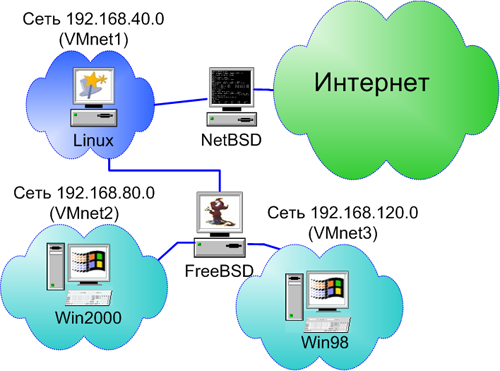
\includegraphics[scale=1]{res/network_general}
\caption{Рабочий макет стандартной схемы ККС.}
\end{figure}

Эмулируемая ККС имеет три сегмента (подсети)\footnote{Адрес подсети должен содержать маску! Далее будем полагать что речь идёт об /24 сетях.}:
\begin{itemize}
\item VMnet1 (адрес подсети – 192.168.40.0)
\item VMnet2 (адрес подсети – 192.168.80.0)
\item VMnet3 (адрес подсети – 192.168.120.0)
\end{itemize}

Сеть VMnet1 содержит основной многофункциональный сервер ККС (службы DHCP, DNS, Web, Proxy, почтовая, файловая и др.), использующий ОС Linux Mandrake. Сеть VMnet2 представлена хостом под управлением ОС Windows 2k (2000/XP/2003 Server) и имеет двойное назначение – она обеспечивает ККС дополнительным сервером и поддерживает Windows-клиент семейства 2k. Сеть VMnet3 объединяет рабочие станции c ограниченными аппаратными ресурсами, ориентированные на ОС Windows семейства 9x (95/98).

Взаимодействие сегментов ККС осуществляет маршрутизатор, обслуживаемый ОС семейства Unix (FreeBSD), а подключение ККС к внешней сети (Интернет или реальной сети учебной лаборатории) обеспечивает шлюз, реализуемый другой ОС семейства Unix (NetBSD).

Естественно, что каждый представитель подсетей (VMnet1, Vmnet2, VMnet3) имеет один сетевой адаптер, шлюз – два, а маршрутизатор – три сетевых адаптера.

Для определённости будем считать, что ККС использует смешанное (и статическое, и динамическое) распределение IP-адресов. 

Хост WIN98 (здесь и далее имя хоста формируется от названия гостевой ОС) имеет статический адрес 192.168.120.15, хост LINUX также имеет статический адрес – 192.168.40.32, а хост WIN2000 получает адрес 192.168.80.128 динамически с помощью виртуального сервера DHCP (встроенного по умолчанию в каждый сегмент сети, эмулируемой в среде VMware Workstation).

\begin{figure}[h!]
\centering
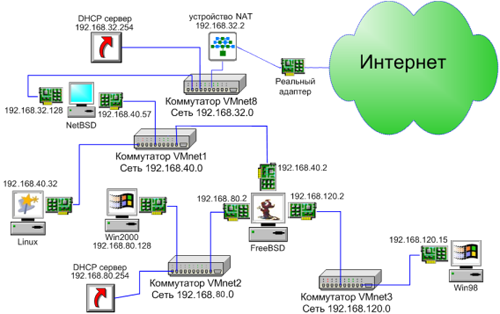
\includegraphics[scale=1]{res/network_general2}
\caption{Стандартная схема ККС.}
\end{figure}

Целесообразно выделить статические адреса для хостов FREEBSD (маршрутизатор) и NETBSD (шлюз). Для простоты адресам всех сетевых адаптеров маршрутизатора назначим одинаковые суффиксы – 192.168.40.2 (для связи с сетью VMnet1), 192.168.80.2 (для связи с сетью VMnet2), 192.168.120.2 (для связи с сетью VMnet3). Функциональное назначение шлюза (обеспечение взаимодействия ККС с внешними сетями) предполагает наличие какого-нибудь механизма сопряжения IP-адресов. Таким механизмом является служба NAT (преобразование сетевых адресов), подключённая к вспомогательной сети VMnet8, в которую (кроме устройства NAT) входит DHCP-сервер и шлюз. Адрес «внешнего» сетевого адаптера шлюза назначается динамически (DHCP-сервером сети VMnet8) – 192.168.32.128, а  адрес «внутреннего» сетевого адаптера шлюза (входящего в сеть VMnet1) статически – 192.168.40.57.

В результате всех подключений имеем схему ККС, представленную на рисунке 2.

%------------------------------------------------------------------------------
\newpage
\section{Эмуляция ККС в среде VirtualBox}

Эмуляция ККС считается завершенной, если выполнены следующие этапы:
\begin{itemize}
\item создание и настройка виртуальных сетей
\item создание и настройка виртуальных хостов
\end{itemize}

\subsection{Создание и настройка виртуальных сетей}

Построим вспомогательную сеть VMnet8 при помощи хост-машины, которая будет через NAT обеспечивать доступ NetBSD к ресурсам сети Интернет.

Для этого в меню File выбираем пункт Preferences, а в открывшемся окне переходим на вкладку Networks (рисунок 3).

\begin{figure}[h!]
\centering
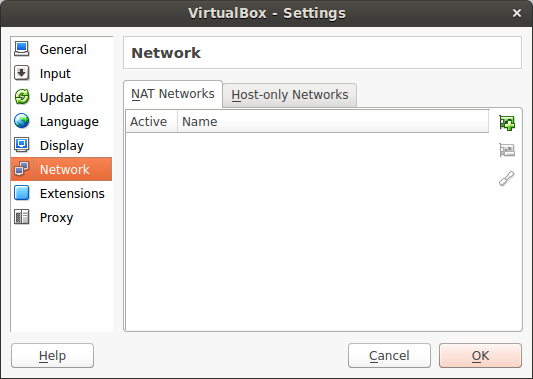
\includegraphics[scale=0.8]{res/virtualbox-networks}
\caption{Настройки сетевой системы VirtualBox.}
\end{figure}

При помощи кнопку со значком "+" добавим новую сетевую карту, которая будет обращена к виртуальной машине, а потом при помощи кнопки с отвёрткой сконфигурируем её так, как показано на рисунке 4.

\begin{figure}[h!]
\centering
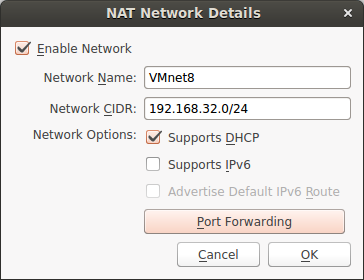
\includegraphics[scale=0.8]{res/virtualbox-nat}
\caption{Подготовка вспомогательной сети VMnet8.}
\end{figure}

Теперь создадим виртуальные машины (без установки и настройки) для прокладки виртуальных сетей. Для начала создадим NetBSD, используя стандартный шаблон, предлагаемый VirtualBox. Далее перейдём в сетевые настройки виртуальной машины и настроим первую сетевую карту для работы в режиме NAT через вспомогательную сеть VMnet8, как показано на рисунке 5.

\begin{figure}[h!]
\centering
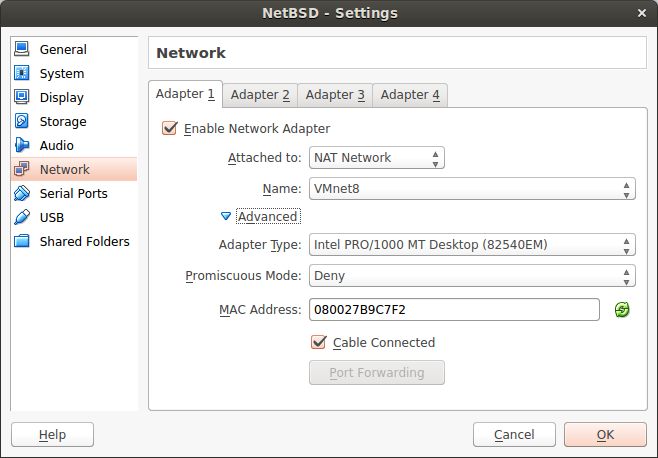
\includegraphics[scale=0.6]{res/netbsd-nat}
\caption{Настройка сетевого интерфейса NetBSD на работу с сетью VMnet8.}
\end{figure}

После этого можно перейти на вкладку с настройками для адаптера 2, включить его и обеспечить подключение к сети VMnet1 (рисунок 6).

\begin{figure}[h!]
\centering
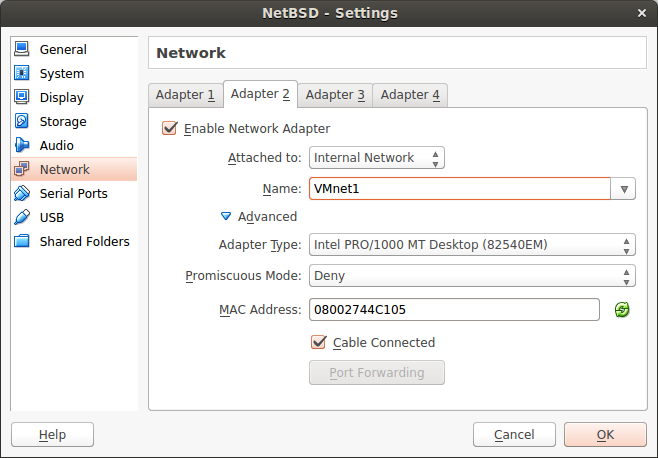
\includegraphics[scale=0.6]{res/netbsd-vmnet1}
\caption{Настройка второго сетевого интерфейса NetBSD на работу с сетью VMnet1.}
\end{figure}

После этого, пользуясь стандартными шаблонами и некоторыми оптимизациями, создадим ещё 4 виртуальные машины (Linux, FreeBSD, Win2000, Win98) и укажем в настройках их сетевых подключений ту сеть, к которой они должны быть подключены (аналогично подключению NetBSD к сети VMnet). При этом машина FreeBSD будет иметь три активированных сетевых адаптера (рисунок 7), и каждый из них будет взаимодействовать со своей виртуальной сетью.

Для организации DHCP в сети VMnet2, к сожалению, нет GUI-инструмента, но эта задача решается через командную строку:

\begin{Verbatim}[frame=single]
VBoxManage dhcpserver add --netname VMnet2 --ip 192.168.40.1 \
   --netmask 255.255.255.0 --lowerip 192.168.40.32 --enable
\end{Verbatim}

Удалить этот DHCP-сервер можно командой

\begin{Verbatim}[frame=single]
VBoxManage dhcpserver remove --netname VMnet2
\end{Verbatim}

\begin{figure}[h!]
\centering
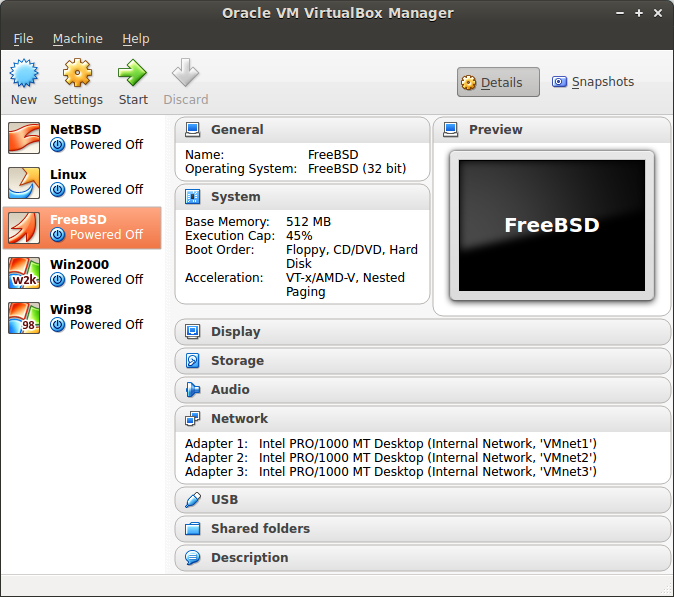
\includegraphics[scale=0.6]{res/freebsd-3net}
\caption{Три сетевые интерфейса, подключенные к разным сетям, на машине FreeBSD.}
\end{figure}

Как можно видеть выше, настройка выделенной виртуальной сети очень проста, для этого нужно только указать её имя. Эта простота компенсируется большей сложностью при создании и удалении DHCP-сервера для этой сети. Возможно в будущих версиях VirtualBox появятся более удобные инструменты для этого.

\newpage
\subsection{Создание и настройка виртуальных хостов}

Для эмуляции ККС требуется пять виртуальных хостов: Win98, Win200, Linux, FreeBSD, NetBSD.

Создание и настройка каждого виртуального хоста состоит из трёх этапов:
\begin{itemize}
\item создание виртуальной машины (этот шаг был проделан в процессе подготовки сети)
\item инсталляция гостевой операционной системы
\item конфигурация хоста в TCP/IP сети
\end{itemize}

Установка будет производиться с ISO-образов дистрибутивов. В целях экономии памяти, предпочтение будет отдаваться 32-х разрядным сборкам.

\subsubsection{Создание и настройка виртуального хоста NetBSD}

Установочный образ NetBSD 6.1.5 (NetBSD-6.1.5-i386.iso) скачиваем с официального сайта \url{http://www.netbsd.org/}.

В процессе установки, система задаст стандартные вопросы, типа предпочитаемого языка, параметров (геометрии) винчестера, желаемого вида установки. Задачей этого хоста является управление сетевым трафиком, следовательно нет необходимости в установке X11.

В процессе установки, система сама (при помощи DHCP) определила параметры интерфейса, который подключен к вспомогательной сети VMnet8 (см. рисунок 8)

\begin{figure}[h!]
\centering
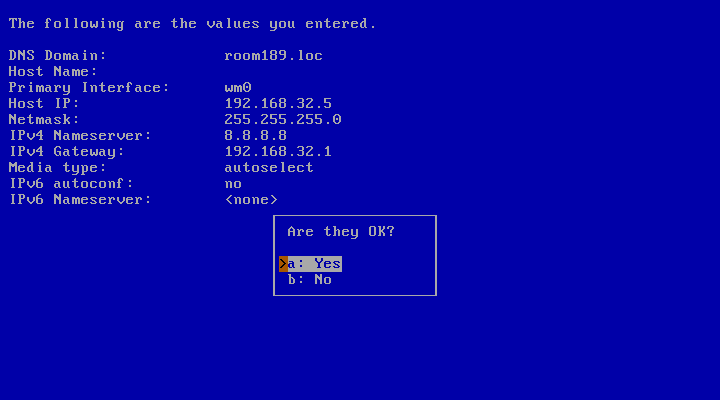
\includegraphics[scale=0.9]{res/netbsd-setup}
\caption{Автоматическое определение параметров сети в NetBSD.}
\end{figure}

После скачивания свежей верирсии портов (изначально wget отсутствует, так что свежие порты можно получить по ftp с \url{ftp.netbsd.org/pub/pkgsrc/stable/pkgsrc.tar.gz}) и установки удобного редактора, можно настроить сеть.

Для настройки второго сетевого интерфейса, в файл /etc/rc.conf нужно добавить строку
\begin{Verbatim}[frame=single]
ifconfig_wm1="inet 192.168.40.57 netmask 255.255.255.0"
\end{Verbatim}

Для включения ip-форвардинга, в файл /etc/sysctl.conf нужно добавить строку
\begin{Verbatim}[frame=single]
net.inet.ip.forwarding=1
\end{Verbatim}

Кроме того, потребовалось настроить некоторые демоны, такие как ipfilter (фаервол работает в режиме полного доступа, т.к. реальные задачи по ограничению доступа должны лежать на машине FreeBSD, выполняющей функции шлюза в локальную сеть) и ipnat (выполняет nat пакетов, предназначенных web-серверу и маскарадинг всех исходящих пакетов).

\begin{figure}[h!]
\centering
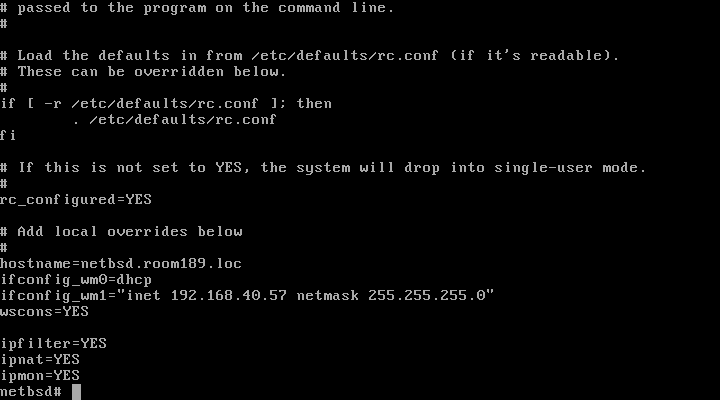
\includegraphics[scale=0.9]{res/netbsd-rcconf}
\caption{Файл инициализации rc.conf в NetBSD.}
\end{figure}

\subsubsection{Создание и настройка виртуального хоста Linux}

Последней версией Mandriva Linux на данный момент является версия 2014.1 (от 26 сентября 2014), установочный образ OpenMandriva.2014.0-kde4.i586.iso. После установки и исправления некоторых ошибок (директория /sbin не попала в переменную окружения \$PATH), выставим IP адрес и проверим работу системы.

Этот хост доступен снаружи по внешнему ip-адресу машины NetBSD, которая перенаправляет запросы, пришедшие на 80-й порт.

На рисунке 10 показана работа Mandriva Linux. В верхней часте экрана присутствует вывод настроек сетевого подключения, в нижней - пинг до DNS-сервера Google.

\begin{figure}[h!]
\centering
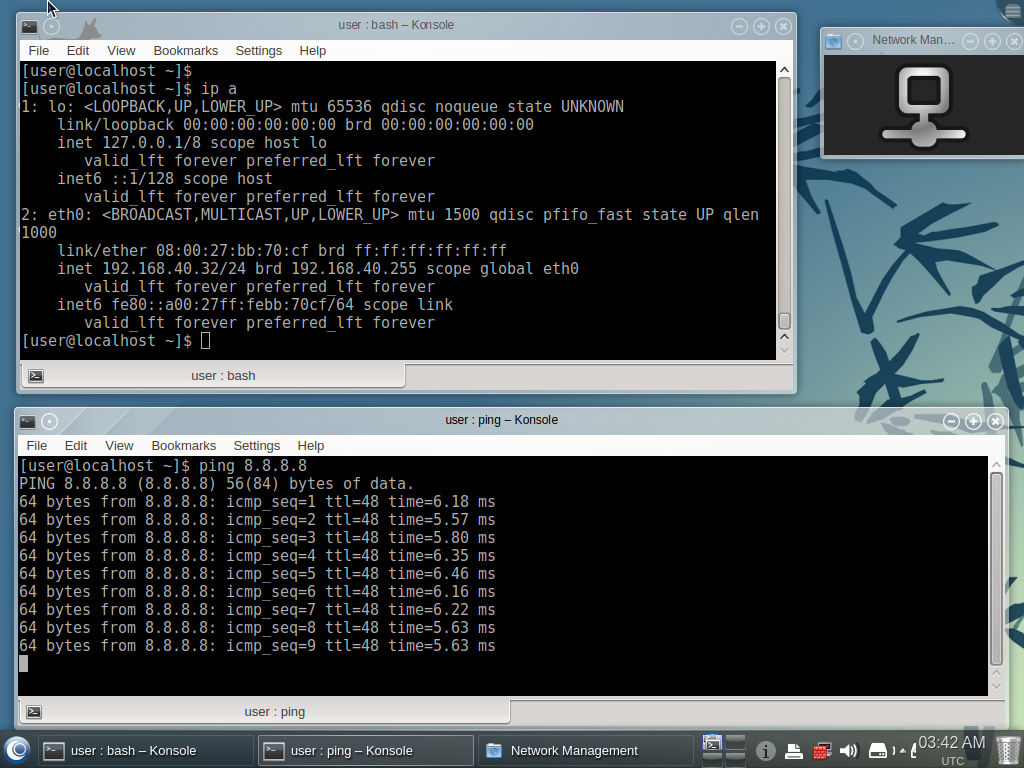
\includegraphics[scale=0.6]{res/linux-general}
\caption{Mandriva linux.}
\end{figure}

Стоит отметить, что в данном случае практически всё работает из коробки, пришлось настроить только IP-адрес. Очевидно, что Mandiva Linux с графической оболочкой KDE не лучший кандидат для корпоративного DHCP, DNS, Web, proxy, почтового и файлового сервера, не говоря уже о том, что эти роли нужно разносить по разным хостам.

\subsubsection{Создание и настройка виртуального хоста FreeBSD}

Как и NetBSD, FreeBSD весьма скромно потребляет ресурсы. В данном примере используется FreeBSD 10.1, установочный образ FreeBSD-10.1-RELEASE-i386-bootonly.iso, т.е. диск позволяет только загрузиться, вся система будет установлена путём скачивания с серверов FreeBSD.

Интересным моментом тут является то, что машина имеет три статически конфигурируемых интерфейса, а для обеспечения доступа из разных подсетей (к примеру, с машины Win98 к машине Win2000) не придётся явно прописывать маршрут, достаточно включить IP-форвардинг. На рисунке 11 представлен вывод файла /etc/rc.conf. Строка gateway\_enable обеспечивает включение форвардинга.

\begin{figure}[h!]
\centering
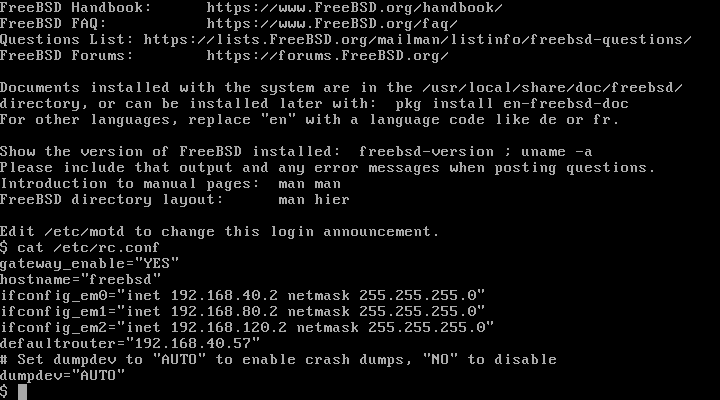
\includegraphics[scale=0.9]{res/freebsd-general}
\caption{FreeBSD.}
\end{figure}

\subsubsection{Создание и настройка виртуального хоста Win2000}

Машина с Windows 2000 получает свой IP динамически, его предоставляет DHCP-сервер, встроенный в VirtualBOox (его работа описывалась ранее).

После этого с Win200 можно отправить пинг на Linux, на все машины, для которых FreeBSD является шлюзом по умолчанию (т.е. это Linux и Win98), а также на саму мушину FreeBSD. Отправка пинга на NetBSD (и далее в интернет) результата не даст, т.к. исходный хост (Win2000) находится в другом широковещательном домене. Чтобы NetBSD знала куда отвечать, на этой машине нужно добавить два маршрута (один для Win2000 и один для Win98):
\begin{Verbatim}[frame=single]
route add -net 192.168.80.0 -netmask 255.255.255.0 192.168.40.2
route add -net 192.168.120.0 -netmask 255.255.255.0 192.168.40.2
\end{Verbatim}

Кроме того, на NetBSD ещё нужно включить NAT для сети VMnet2 и VMnet3:
\begin{Verbatim}[frame=single]
echo "map wm0 192.168.80.0/24 -> 192.168.32.5/32" >> /etc/ipnat.conf
echo "map wm0 192.168.120.0/24 -> 192.168.32.5/32" >> /etc/ipnat.conf
\end{Verbatim}

В результате Win2000 может общаться с внешним миром. На рисунке 12 в верхней часте отображены текущие сетевые настройки машины, в левой части пинг на DNS-сервер гугла (8.8.8.8; пакет идёт через трансляцию сетевых адресов на NetBSD), а в правой - пинг на win98 (пакет идёт через FreeBSD и для этого не потребовалось никаких настроек роутинга).

\begin{figure}[h!]
\centering
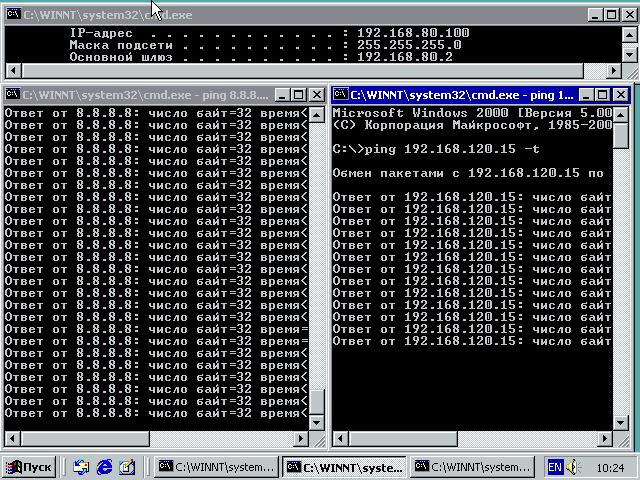
\includegraphics[scale=1]{res/win2000-general}
\caption{Win2000.}
\end{figure}

\subsubsection{Создание и настройка виртуального хоста Win98}

Ситуация с Win98 фактически аналогична ситуации с Win2000: эта машина также может отправлять пакеты всем хостам, для которых FreeBSD является шлюзом по умолчанию (и самой машине FreeBSD), а после дополнительных настроек маршрутизации и сетевой трансляции (рассмотренных выше) - отправлять пакеты в интернет.

Машина с Win98 получает свой адрес статически (рисунок 13).

\begin{figure}[h!]
\centering
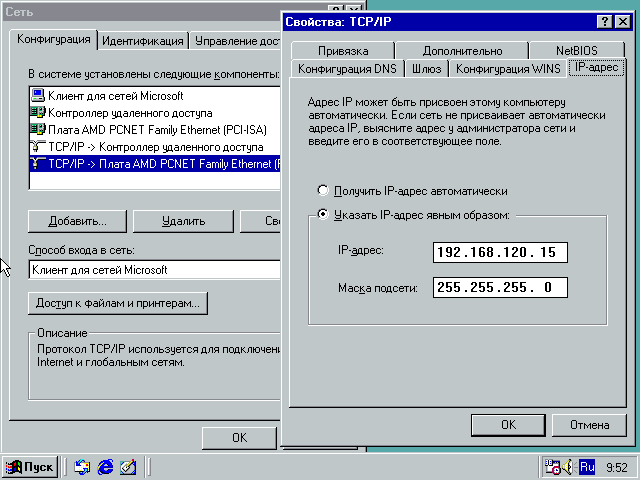
\includegraphics[scale=0.9]{res/win98-general}
\caption{Win98.}
\end{figure}